\documentclass[crop, tikz]{standalone}
\usepackage{tikz}
\usepackage{relsize}
\usepackage{bm}

\usetikzlibrary{positioning,decorations.pathmorphing}

\definecolor{mygreen}{rgb}{0,0.6,0}
\definecolor{mymauve}{rgb}{0.58,0,0.82} 
\definecolor{camdrk}{RGB}{0,62,114}

\begin{document}
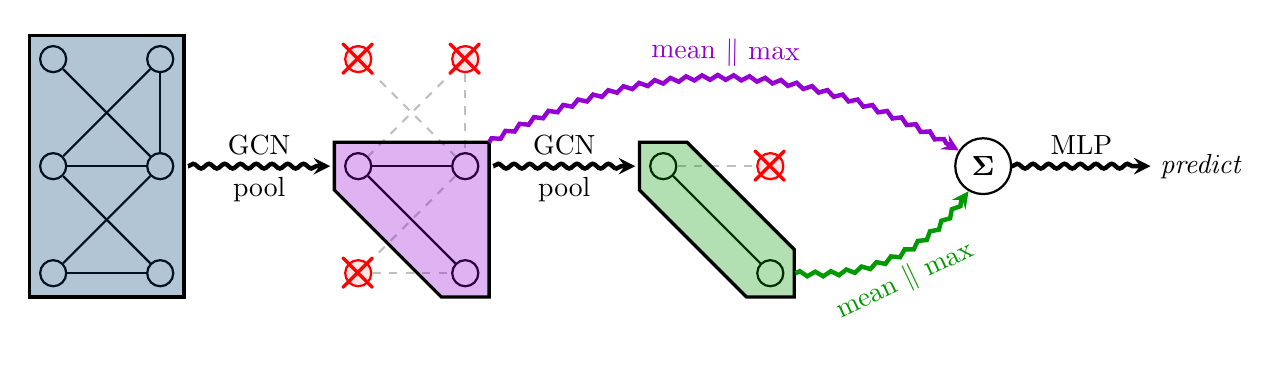
\begin{tikzpicture}

	\node[circle, draw, thick] (h1) {};
	\node[circle, draw, thick, right=of h1] (h2) {};
	\node[circle, draw, thick, below=of h1] (h3) {};
	\node[circle, draw, thick, right=of h3] (h4) {};
	\node[circle, draw, thick, below=of h3] (h5) {};
	\node[circle, draw, thick, right=of h5] (h6) {};

	\draw[-, thick] (h1) -- (h4);
	\draw[-, thick] (h2) -- (h3);
	\draw[-, thick] (h2) -- (h4);
	\draw[-, thick] (h3) -- (h4);
	\draw[-, thick] (h3) -- (h6);
	\draw[-, thick] (h4) -- (h5);
	\draw[-, thick] (h5) -- (h6);
	
	\path [draw=black, smooth, fill=camdrk, fill opacity=0.3, very thick]
       ([xshift=-0.5em,yshift=0.5em]h1.north west) -- ([xshift=0.5em,yshift=0.5em]h2.north east) -- ([xshift=0.5em,yshift=-0.5em]h6.south east) -- ([xshift=-0.5em,yshift=-0.5em]h5.south west) -- cycle;
	
	\node[circle, draw, thick, red, fill=red!10, right=10em of h1] (g1) {};
	\node[circle, draw, thick, red, fill=red!10, right=of g1] (g2) {};
	\node[circle, draw, thick, below=of g1] (g3) {};
	\node[circle, draw, thick, right=of g3] (g4) {};
	\node[circle, draw, thick, red, fill=red!10, below=of g3] (g5) {};
	\node[circle, draw, thick, right=of g5] (g6) {};

	\draw[-, thick, dashed, lightgray] (g1) -- (g4);
	\draw[-, thick, dashed, lightgray] (g2) -- (g3);
	\draw[-, thick, dashed, lightgray] (g2) -- (g4);
	\draw[-, thick] (g3) -- (g4);
	\draw[-, thick] (g3) -- (g6);
	\draw[-, thick, dashed, lightgray] (g4) -- (g5);
	\draw[-, thick, dashed, lightgray] (g5) -- (g6);
	
	\node[red] (icr) at (g1) {$\mathlarger{\mathlarger{\mathlarger{\mathlarger{\mathlarger{\bm{\times}}}}}}$};
	\node[red] (icr) at (g2) {$\mathlarger{\mathlarger{\mathlarger{\mathlarger{\mathlarger{\bm{\times}}}}}}$};
	\node[red] (icr) at (g5) {$\mathlarger{\mathlarger{\mathlarger{\mathlarger{\mathlarger{\bm{\times}}}}}}$};

	\path [draw=black, smooth, fill=mymauve, fill opacity=0.3, very thick]
       ([xshift=-0.5em,yshift=0.5em]g3.north west) -- ([xshift=0.5em,yshift=0.5em]g4.north east) -- ([xshift=0.5em,yshift=-0.5em]g6.south east) -- ([xshift=-0.5em,yshift=-0.5em]g6.south west) -- ([xshift=-0.5em,yshift=-0.5em]g3.south west) -- cycle;
	
	\node[circle, thick, right=10em of g1] (i1) {};
	\node[circle, thick, right=of i1] (i2) {};
	\node[circle, draw, thick, below=of i1] (i3) {};
	\node[circle, draw, red, thick, fill=red!10, right=of i3] (i4) {};
	\node[circle, thick, below=of i3] (i5) {};
	\node[circle, draw, thick, right=of i5] (i6) {};

	\draw[-, thick, dashed, lightgray] (i3) -- (i4);
	\draw[-, thick] (i3) -- (i6);
	
	\node[red] (icr) at (i4) {$\mathlarger{\mathlarger{\mathlarger{\mathlarger{\mathlarger{\bm{\times}}}}}}$};
	
	\draw[-stealth, ultra thick,decoration={snake, pre length=0.01mm, segment length=2mm, amplitude=0.3mm, post length=1.5mm}, decorate] ([xshift=0.5em]h4.east) -- node[below, black] {pool} node[above] {GCN} ([xshift=-0.5em]g3.west);
	\draw[-stealth, ultra thick,decoration={snake, pre length=0.01mm, segment length=2mm, amplitude=0.3mm, post length=1.5mm}, decorate] ([xshift=0.5em]g4.east) -- node[above] {GCN} node[below] {pool}([xshift=-0.5em]i3.west);
	
	\path [draw=black, smooth, fill=mygreen, fill opacity=0.3, very thick]
       ([xshift=-0.5em,yshift=0.5em]i3.north west) -- ([xshift=0.5em,yshift=0.5em]i3.north east) --([xshift=0.5em,yshift=0.5em]i6.north east) --([xshift=0.5em,yshift=-0.5em]i6.south east) -- ([xshift=-0.5em,yshift=-0.5em]i6.south west) -- ([xshift=-0.5em,yshift=-0.5em]i3.south west) -- cycle;
       
    \node[circle, draw, thick, right=10em of i3] (S) {$\boldsymbol\Sigma$};
    
    \path[-stealth, mymauve, ultra thick] ([xshift=0.5em, yshift=0.5em]g4.north east) edge[bend left,decoration={zigzag, pre length=0.01mm, segment length=2mm, amplitude=0.3mm, post length=1.5mm}, decorate] node[sloped,above] {mean $\|$ max} (S);
    
	
    \path[-stealth, mygreen, ultra thick] ([xshift=0.4em]i6.east) edge[bend right,decoration={zigzag, pre length=0.01mm, segment length=2mm, amplitude=0.3mm, post length=1.5mm}, decorate] node[sloped,below] {mean $\|$ max} (S);
    
    \node[right=5em of S] (P) {\emph{predict}};
    
	\draw[-stealth, ultra thick,decoration={snake, pre length=0.01mm, segment length=2mm, amplitude=0.3mm, post length=1.5mm}, decorate] (S.east) --node[above] {MLP} (P.west);
	
\end{tikzpicture}
\end{document}